\documentclass[tikz,border=3mm]{standalone}
\usepackage{amsmath,amssymb}
\usetikzlibrary{arrows.meta,positioning,shapes.geometric,fit,backgrounds}
\begin{document}
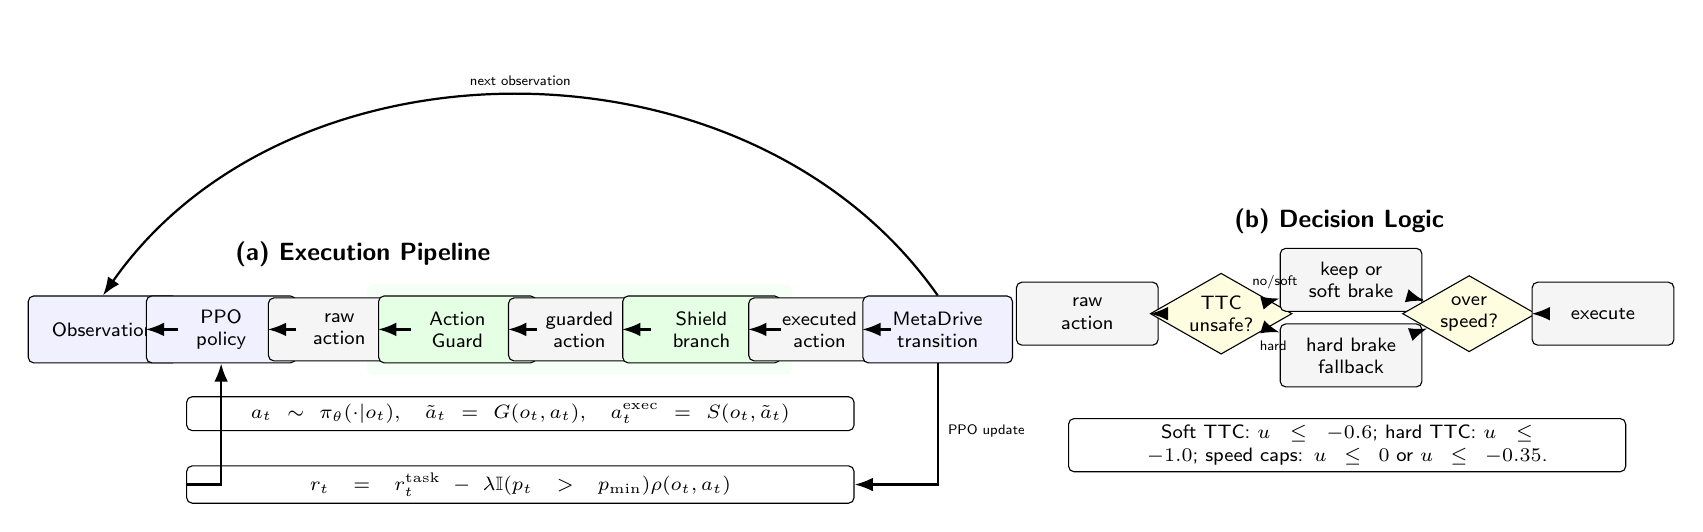
\begin{tikzpicture}[font=\sffamily, >=Latex,
box/.style={draw, rounded corners=2pt, fill=blue!6, minimum width=19mm, minimum height=8.5mm, align=center, font=\sffamily\scriptsize},
safe/.style={draw, rounded corners=2pt, fill=green!10, minimum width=20mm, minimum height=8.5mm, align=center, font=\sffamily\scriptsize},
act/.style={draw, rounded corners=2pt, fill=gray!8, minimum width=18mm, minimum height=8mm, align=center, font=\sffamily\scriptsize},
decide/.style={draw, diamond, aspect=1.75, fill=yellow!12, inner sep=1.0pt, align=center, font=\sffamily\scriptsize},
formula/.style={draw, rounded corners=2pt, fill=white, inner sep=2.5pt, align=center, font=\sffamily\scriptsize}]

\node[font=\sffamily\bfseries\small] at (-2.95,1.20) {(a) Execution Pipeline};
\node[box] (obs) at (-6.25,0.25) {Observation};
\node[box] (ppo) at (-4.75,0.25) {PPO\\policy};
\node[act] (raw) at (-3.25,0.25) {raw\\action};
\node[safe] (guard) at (-1.75,0.25) {Action\\Guard};
\node[act] (gact) at (-0.20,0.25) {guarded\\action};
\node[safe] (shield) at (1.35,0.25) {Shield\\branch};
\node[act] (exec) at (2.85,0.25) {executed\\action};
\node[box] (env) at (4.35,0.25) {MetaDrive\\transition};
\node[formula, text width=83mm] (eq) at (-0.95,-0.82) {$a_t\sim\pi_\theta(\cdot|o_t),\quad \tilde a_t=G(o_t,a_t),\quad a_t^{\rm exec}=S(o_t,\tilde a_t)$};
\node[formula, text width=83mm] (rw) at (-0.95,-1.72) {$r_t=r_t^{\rm task}-\lambda\mathbb{I}(p_t>p_{\min})\rho(o_t,a_t)$};
\draw[->, thick] (obs) -- (ppo);
\draw[->, thick] (ppo) -- (raw);
\draw[->, thick] (raw) -- (guard);
\draw[->, thick] (guard) -- (gact);
\draw[->, thick] (gact) -- (shield);
\draw[->, thick] (shield) -- (exec);
\draw[->, thick] (exec) -- (env);
\draw[->, thick, rounded corners=8pt] (env.north) to[out=125,in=55] node[above,font=\sffamily\tiny] {next observation} (obs.north);
\draw[->, thick] (env.south) |- node[pos=0.28,right,font=\sffamily\tiny] {PPO update} (rw.east);
\draw[->, thick] (rw.west) -| (ppo.south);
\begin{scope}[on background layer]
\node[fill=green!4, rounded corners=2pt, fit=(guard)(shield), inner sep=4pt] {};
\end{scope}

\node[font=\sffamily\bfseries\small] at (9.45,1.62) {(b) Decision Logic};
\node[act] (r0) at (6.25,0.45) {raw\\action};
\node[decide] (r1) at (7.95,0.45) {TTC\\unsafe?};
\node[act] (r2) at (9.60,0.88) {keep or\\soft brake};
\node[act] (r3) at (9.60,-0.08) {hard brake\\fallback};
\node[decide] (r4) at (11.10,0.45) {over\\speed?};
\node[act] (r5) at (12.80,0.45) {execute};
\node[formula, text width=69mm] at (9.55,-1.22) {Soft TTC: $u\le -0.6$; hard TTC: $u\le -1.0$; speed caps: $u\le 0$ or $u\le -0.35$.};
\draw[->, thick] (r0) -- (r1);
\draw[->, thick] (r1) -- node[above,font=\sffamily\tiny] {no/soft} (r2);
\draw[->, thick] (r1) -- node[below,font=\sffamily\tiny] {hard} (r3);
\draw[->, thick] (r2) -- (r4);
\draw[->, thick] (r3) -- (r4);
\draw[->, thick] (r4) -- (r5);
\end{tikzpicture}
\end{document}
